\section{Results on the DIPSER slice and transfer}
\label{sec:results}

\subsection{Fusion versus the best single stream (Q1)}
Fig.~\ref{fig:slice} shows the 33 configurations of the slice, and Supplementary Table~S1 lists them. The best single stream is the face mesh trained with the soft target (QWK $0.256\pm0.068$). The best fusion (gate, link on, dropout off, soft target) reaches $0.124\pm0.071$ and the best core fusion $0.113\pm0.073$. On identical folds, the best fusion falls short of the best single stream by $0.327$, $0.046$ and $0.021$ for the three seeds (mean $0.131$), so the size of the mean gap is driven by one seed. Only 1 of the 72 seed-level fusion results exceeds the best single stream of the same seed, and 14 of the 24 configurations score at or below zero.

Among the single streams, only the mesh carries signal on the slice (QWK $0.256$, against $0.003$ for the image stream, $0.002$ for physiology and $0.002$ for head pose, each with its better objective). The permuted-label control stays at $0.009\pm0.018$. Decision-level voting over the four single-stream predictions performs no better than feature-level fusion ($0.011\pm0.047$ and $0.006\pm0.028$ for streams trained with the soft and the CORAL objective).

\begin{figure}[!t]
\centering
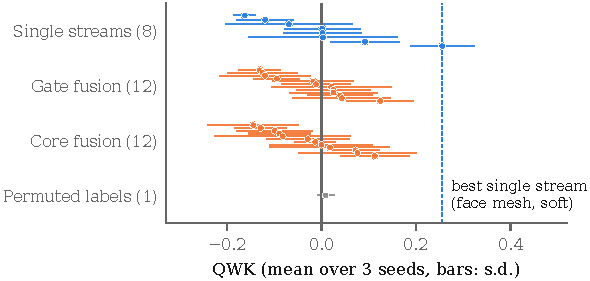
\includegraphics[width=\columnwidth]{figures/fig_slice_grid.pdf}
\caption{DIPSER slice (1{,}566 complete windows, folds grouped by student-session). Each point is one configuration: pooled out-of-fold QWK, mean over three seeds; bars show the standard deviation over seeds. The dashed line marks the best single stream.}
\label{fig:slice}
\end{figure}

\subsection{Gate, global link and dropout (Q2, Q3)}
Table~\ref{tab:contrasts} reports the paired contrasts. The gate ends one-hot (weight $\ge0.98$ on one stream) in 108 of the 180 gated fits (60\%), and it selects the mesh stream, the only informative one, in 41 of them. Gate and core fusion do not differ significantly (gate better in 7 of 12 pairs, median difference $-0.009$, $p=0.68$); the same holds on DAiSEE ($p=0.46$ under P1 and $0.95$ under P2).

The global link improves QWK on the slice in 10 of 12 pairs (median $+0.076$, $p=0.002$). At initialisation it makes the gradient that reaches the first tower layers 12 to 132 times larger; these probes use a single seed and fold and do not establish the mechanism. On DAiSEE the effect is reversed: the link improves 0 of 8 pairs under P1 and 1 of 8 under P2 (median $-0.046$ and $-0.024$; $p=0.008$ and $0.016$). A possible explanation is that the link gives the head direct access to high-dimensional inputs that carry little signal on that dataset; we did not test it. Modality dropout has no reliable effect (better in 8 of 12 pairs, median $-0.016$, $p=0.62$).

\begin{table*}[!t]
\centering
\caption{Paired contrasts between configurations that differ in one factor. Wins: pairs in which the first level has the higher mean QWK. Med./Mean $\Delta$: median and mean per-seed QWK differences. $p_{\text{cfg}}$: Wilcoxon signed-rank test on configuration-level means (primary); $p_{\text{seed}}$: on per-seed differences (secondary). Values are not corrected for multiple comparisons; see Section~\ref{sec:threats}.}
\label{tab:contrasts}
\small
\setlength{\tabcolsep}{3pt}
\begin{tabular}{llccccc}
\toprule
Contrast & Data & Wins & Med. $\Delta$ & Mean $\Delta$ & $p_{\text{cfg}}$ & $p_{\text{seed}}$ \\
\midrule
\csname @@input\endcsname tables/contrasts.tex
\bottomrule
\end{tabular}
\end{table*}

\subsection{Ordinal objectives (Q4)}
In the fusion configurations the soft target outperforms CORAL in 7 of 8 pairs (median $+0.062$, $p=0.023$) and the hybrid objective in 7 of 8 ($+0.117$, $p=0.016$). By the proposition of Section~\ref{sec:instrument}, a difference between soft and CORAL can only come from rater disagreement. The evidence is nevertheless weak. After a Holm correction over the slice contrasts only the link remains significant ($p=0.012$; soft against CORAL, $p=0.070$), on person-disjoint windows the soft target wins 6 of 8 pairs without significance ($p=0.078$), and for single streams it wins 2 of 4 pairs. For the mesh stream it raises QWK from $0.092$ to $0.256$, and for the image stream from $-0.163$ to $0.003$.

Zeroing one stream at inference harms both fusion types, most strongly the mesh stream for the gate ($-0.129$) and the image stream for core fusion ($-0.111$). On the high level, which has seven windows, recall is 0.00 for the best single stream and 0.19 for the best fusion, which over-predicts this level; 81--99\% of the errors are one level off.

\subsection{Transfer to DAiSEE and EngageNet (Q5)}
Table~\ref{tab:transfer} gives the transfer results. Fusion yields no meaningful gain over the best single stream on DAiSEE ($+0.010$ under P2 and $-0.001$ under P1), and it trails it on the EngageNet frames (gate $0.170$ against mesh $0.366$). The permuted controls remain near zero ($0.024$ and $0.035$). The informative stream differs between datasets: the mesh leads on DIPSER and on EngageNet, whereas on DAiSEE the image stream (P1, $0.093$) and the head pose (P2, $0.050$) lead, and no configuration exceeds QWK $0.10$.

\begin{table*}[!t]
\centering
\caption{Transfer: pooled QWK (mean $\pm$ s.d. over three seeds). $\Delta$: best fusion minus best single stream. Perm.: permuted-label control. $^\dagger$Reduced set of configurations, frame-level samples, P2 only.}
\label{tab:transfer}
\small
\setlength{\tabcolsep}{2.5pt}
\begin{tabular}{lcccccc}
\toprule
Setting & Image & Mesh & Pose & Best fusion & $\Delta$ & Perm. \\
\midrule
\csname @@input\endcsname tables/transfer.tex
\bottomrule
\end{tabular}
\end{table*}

\textbf{Position with respect to published DAiSEE results.} Table~\ref{tab:comparison} places the instrument beside published systems on the official test set. On that set, the best single stream (image stream, CORAL, selected on Validation) obtains QWK $0.043\pm0.013$ at 50.4\% accuracy and the best fusion $0.044\pm0.018$, while the majority predictor reaches 51.8\% on the clips we score. Published studies report accuracy and no QWK, but three of them print a test confusion matrix, from which we derive QWK values between \pubResTcnQwk{} and \pubOrdTcnQwk. With a training-free moment front-end and six frames per clip, the instrument is therefore far below systems that use learned spatio-temporal features on DAiSEE, and its DAiSEE results should be read only as a within-instrument comparison of fusion against single streams. The table also shows the limits of accuracy on this dataset: the lowest level has four test clips, so that its recall can only be 0 or a multiple of 0.25, and the system with the highest accuracy among those with a printed matrix has a recall of \pubOrdTcnRecOne{} on the second level (84 clips).

\begin{table}[!t]
\centering
\caption{DAiSEE, four classes, official test set. Published rows: single reported runs on 1{,}784 clips (majority rate \pubMajority\%). Our rows: mean over three seeds on the 1{,}638 clips with all streams (P1-Test). Rec.\,0 and Rec.\,1: recall of the two lowest levels (4 and 84 clips in the full test set). $^\ast$Derived by us from the published confusion matrix; n.r.: not reported and not derivable.}
\label{tab:comparison}
\footnotesize
\setlength{\tabcolsep}{2pt}
\begin{tabular}{lcccc}
\toprule
Method & Acc.\,\% & Rec.\,0 & Rec.\,1 & QWK \\
\midrule
DFSTN~\cite{liao2021dfstn} & 58.84 & n.r. & n.r. & n.r. \\
ResNet+TCN~\cite{abedi2021resnettcn} & 63.9 & 0.00$^\ast$ & \pubResTcnRecOne$^\ast$ & \pubResTcnQwk$^\ast$ \\
Ordinal TCN~\cite{abedi2024affectordinal} & 67.4 & 0.25$^\ast$ & \pubOrdTcnRecOne$^\ast$ & \pubOrdTcnQwk$^\ast$ \\
Contrastive ordinal~\cite{abedi2025supervised} & 67.32 & 0.00 & \pubContrastiveRecOne & \pubContrastiveQwk$^\ast$ \\
ViBED-Net (preprint)~\cite{gothwal2025vibednet} & 73.43 & 0.25 & 0.79 & n.r. \\
\midrule
Majority (1{,}638 clips) & 51.8 & 0.00 & 0.00 & 0.00 \\
gTAO-Net, best single stream & 50.4 & 0.00 & 0.02 & $0.043\pm0.013$ \\
gTAO-Net, best fusion & 50.2 & 0.00 & 0.01 & $0.044\pm0.018$ \\
\bottomrule
\end{tabular}
\end{table}

\textbf{Computational cost.} The 495 fits of the slice train in 24 minutes on a Kaggle GPU and in an estimated 15--18 minutes on a laptop CPU; the GPU brings no speed-up for models of 1.12 to 2.07 million parameters (Supplementary Table~S2). Tchebichef encoding takes 0.6\,ms per window.
